\documentclass[slovene,11pt,a4paper]{article}
\usepackage[margin=2cm,bottom=2cm,foot=1.5cm]{geometry}
% \documentclass[slovene,11pt,a4paper]{article}
% \usepackage[margin=1.7cm,bottom=3cm,foot=1.5cm]{geometry}
\setlength{\parindent}{0pt}
\setlength{\parskip}{0.5ex}

\usepackage[pdftex]{graphicx}
\usepackage{pgffor}
\usepackage{subcaption}
% \usepackage{a4wide} %najaci package
\usepackage[utf8]{inputenc}
\usepackage[slovene]{babel}
\usepackage{color}
\usepackage{graphicx}
% \usepackage{subfigure}
\usepackage{imakeidx}
\usepackage{adjustbox}
\usepackage{float}
\usepackage{amsmath}
\usepackage{mathtools}
\usepackage{tikz}
\usepackage{amssymb}
\usepackage{listings}
\usepackage{siunitx}
\usepackage{hyperref}
\usepackage{amsfonts}
\usepackage{mathrsfs}


%\def\phi{\phi}
\def\eps{\varepsilon}
\def\theta{\vartheta}

\newcommand{\thisyear}{2024/25}

\renewcommand{\Re}{\mathop{\rm Re}\nolimits}
\renewcommand{\Im}{\mathop{\rm Im}\nolimits}
\newcommand{\Tr}{\mathop{\rm Tr}\nolimits}
\newcommand{\diag}{\mathop{\rm diag}\nolimits}
\newcommand{\dd}{\,\mathrm{d}}
\newcommand{\ddd}{\mathrm{d}}
\newcommand{\ii}{\mathrm{i}}
\newcommand{\lag}{\mathcal{L}\!}
\newcommand{\ham}{\mathcal{H}\!}
\newcommand{\four}[1]{\mathcal{F}\!\left(#1\right)}
\newcommand{\bigO}[1]{\mathcal{O}\!\left(#1\right)}
\newcommand{\sh}{\mathop{\rm sinh}\nolimits}
\newcommand{\ch}{\mathop{\rm cosh}\nolimits}
\renewcommand{\th}{\mathop{\rm tanh}\nolimits}
\newcommand{\erf}{\mathop{\rm erf}\nolimits}
\newcommand{\erfc}{\mathop{\rm erfc}\nolimits}
\newcommand{\sinc}{\mathop{\rm sinc}\nolimits}
\newcommand{\rect}{\mathop{\rm rect}\nolimits}
\newcommand{\ee}[1]{\cdot 10^{#1}}
\newcommand{\inv}[1]{\left(#1\right)^{-1}}
\newcommand{\invf}[1]{\frac{1}{#1}}
\newcommand{\sqr}[1]{\left(#1\right)^2}
\newcommand{\half}{\frac{1}{2}}
\newcommand{\thalf}{\tfrac{1}{2}}
\newcommand{\pd}{\partial}
\newcommand{\Dd}[3][{}]{\frac{\ddd^{#1} #2}{\ddd #3^{#1}}}
\newcommand{\Pd}[3][{}]{\frac{\pd^{#1} #2}{\pd #3^{#1}}}
\newcommand{\avg}[1]{\left\langle#1\right\rangle}
\newcommand{\norm}[1]{\left\Vert #1 \right\Vert}
\newcommand{\braket}[2]{\left\langle #1 \vert#2 \right\rangle}
\newcommand{\obraket}[3]{\left\langle #1 \vert #2 \vert #3 \right \rangle}
\newcommand{\hex}[1]{\texttt{0x#1}}

\renewcommand{\iint}{\mathop{\int\mkern-13mu\int}}
\renewcommand{\iiint}{\mathop{\int\mkern-13mu\int\mkern-13mu\int}}
\newcommand{\oiint}{\mathop{{\int\mkern-15mu\int}\mkern-21mu\raisebox{0.3ex}{$\bigcirc$}}}

\newcommand{\wunderbrace}[2]{\vphantom{#1}\smash{\underbrace{#1}_{#2}}}

\newcommand{\bec}[1]{\mathbf{#1}}

\title{
\sc\large Matematično-fizikalni praktikum\\
\bigskip
\bf\Large 12.~naloga: Strojno učenje (machine learning)
}
\author{Tadej Tomažič}
\date{}
\makeindex[columns=3, title=Alphabetical Index, intoc]

\begin{document}
\pagenumbering{gobble} 
\author{Tadej Tomažič}
\date{\today}

\maketitle

\newpage
\pagenumbering{arabic}
\tableofcontents
\listoffigures
\newpage
\vspace{-1cm}
\section{Navodilo}
\vspace{-1cm}

Dandanes je uporaba različnih algoritmov strojnega učenja (Machine Learning, ML) v 
znanosti že rutinsko opravilo. Poznamo tri osnovne vrste stojnega učenja:
\begin{itemize}
  \item Nadzorovano učenje (Supervised learning):
  \begin{itemize}
    \item Klasifikacija (Classification): sortiranje v različne kategorije.
    \item Regresija (Regression): modeliranje oz. `fitanje' napovedi.
  \end{itemize}
  \item Nenadzorovano učenje ( npr. sam najdi kategorije).
  \item Stimulirano učenje ( Artificial Intelligence v ožjem pomenu besede).
\end{itemize}
V fiziki (in tej nalogi), se tipično ukvarjamo s prvo kategorijo, bodisi za identifikacijo novih pojavov/delcev/\ldots ali pa za ekstrakcijo napovedi (netrivialnih funkcijskih odvisnosti etc).

ML algoritmi imajo prednost pred klasičnim pristopom, da lahko učinkovito razdrobijo kompleksen problem na enostavne elemente in ga ustrezno opišejo:
\begin{itemize}
  \item pomisli na primer, kako bi bilo težko kar predpostaviti/uganiti 
  pravo analitično funkcijo v več dimenzijah ( in je npr. uporaba zlepkov 
  (spline interpolacija) mnogo lažja in boljša ).
  \item Pri izbiri/filtriranju velike količine podatkov z mnogo lastnostmi 
  (npr dogodki pri trkih na LHC) je zelo težko najti količine, ki optimalno 
  ločijo signal od ozadnja, upoštevati vse korelacije in najti optimalno kombinacijo 
  le-teh\ldots
\end{itemize} 

Če dodamo malce matematičnega formalizma strojnega učenja: Predpostavi, da imamo na voljo nabor primerov 
\(\mathcal{D}=\left\{\left(\mathbf{x}_{k}, y_{k}\right)\right\}_{k=1 . N},\) kjer je
\(\mathbf{x}_{k}=\left(x_{k}^{1}, \ldots, x_{k}^{M}\right)\) naključno izbrani vektor
 \(M\) lastnosti (karakteristik) in je \(\mathbf{y}_{k} = \left(y_{k}^{1}, \ldots, y_{k}^{Q}\right)\)
 vektor $Q$ ciljnih vrednosti, ki so lahko bodisi binarne ali pa realna 
 števila\footnote{...ali pa še kaj, prevedljive na te možnosti, npr barve\ldots}. 
 Vrednosti \(\left(\mathbf{x}_{k}, \mathbf{y}_{k}\right)\) so neodvisne in porazdeljene po neki
 neznani porazdelitvi \(P(\cdot, \cdot) .\) Cilj ML metode je določiti (priučiti) funkcijo
 \(h: \mathbb{R}^{Q} \rightarrow \mathbb{R}\), ki minimizira pričakovano vrednost \emph{funkcije
 izgube (expected loss)} \[\mathcal{L}(h)=\mathbb{E}\, L(\mathbf{y}, \mathbf{h}(\mathbf{x})) = \frac{1}{N}\sum\limits_{k=1}^{N} L(\mathbf{y_k}, \mathbf{h}(\mathbf{x_k}))  .\] 
 Tu je \(L(\cdot, \cdot)\)  gladka funkcija, ki opisuje oceno za kvaliteto napovedi, 
 pri čemer so  vrednosti \((\mathbf{x}, \mathbf{y})\)
 neodvisno  vzorčene iz nabora \(\mathcal{D}\) po porazdelitvi \(P\). Po koncu učenja
 imamo torej na voljo funkcijo $\mathbf{h}(\mathbf{x})$, ki nam za nek vhodni nabor vrednosti
 $\mathbf{\hat{x}}$ poda napoved $\mathbf{\hat{y}}=\mathbf{h}(\mathbf{\hat{x}})$, ki ustrezno kategorizira
 ta nabor vrednosti. 
 
 Funkcije $\mathbf{h}$ so v praksi sestavljene iz (množice) preprostih funkcij z (nekaj) prostimi
 parametri, kar na koncu seveda pomeni velik skupni nabor neznanih parametrov in zahteven
 postopek minimizacije funkcije izgube. 
 
 Osnovni gradnik odločitvenih dreves je tako kar stopničasta funkcija $H(x_i-t_i)={0,1}$, ki je enaka
 ena za $x_i > t_i$ in nič drugače in kjer je $x_i$ ena izmed karakteristik in $t_i$ neznani parameter.
Iz skupine takšnih funkcij, ki predstavljajo binarne odločitve lahko skonstruiramo končno uteženo 
funkcijo \[\mathbf{h}(\mathbf{x})=\sum\limits_{i=1}^{J} \mathbf{a}_{i}\, H(x_i-t_i),\] kjer so $\mathbf{a}_i$ vektorji neznanih uteži. 
Tako $t_i$ kot $\mathbf{b}_i$, lahko določimo v procesu učenja. Nadgradnjo predstavljajo nato \emph{pospešena} odločitvena
drevesa (BDT), kjer nadomestimo napoved enega drevesa z uteženo množico le-teh, tipično dobljeno
v ustreznih iterativnih postopkih (npr. AdaBoost, Gradient Boost ipd.).

Pri nevronskih mrežah je osnovni gradnik t.i. \emph{perceptron}, ki ga opisuje preprosta funkcija
\[h_{w,b}(\mathbf{X})=\operatorname{\theta}\left(\mathbf{w}^{T} \cdot \mathbf{X} + b\right),\]
kjer je $\mathbf{X}$ nabor vhodnih vrednosti, $\mathbf{w}$ vektor vrednosti uteži, s katerimi
tvorimo uteženo vsoto ter $b$ dodatni konstatni premik (bias). Funkcija $\theta$ je preprosta
gladka funkcija (npr. $\arctan$), ki lahko vpelje nelinearnost v odzivu perceptrona. Nevronska
mreža je nato sestavljena iz (poljubne) topologije takšnih perceptronov, ki na začetku
sprejme karakteristiko dogodka $\mathbf{x}$ v končni fazi rezultirajo v napovedi $\mathbf{\hat{y}}$, ki 
mora seveda biti čim bližje ciljni vrednosti $\mathbf{y}$. Z uporabo ustrezne funkcije 
izgube (npr MSE: \(\mathcal{L}(h)=\mathbb{E}\, ||\mathbf{y}-\mathbf{\hat{y}}||^2\)), se problem znova prevede na
minimizacijo, kjer iščemo optimalne vrednosti (velikega) nabora uteži $\mathbf{w}_i$ ter
$b_i$ za vse perceptrone v mreži. Globoke nevronske mreže (DNN) niso nič drugega, kot 
velike nevronske mreže ali skupine le-teh. 

Že namizni računalniki so
dovolj močni za  osnovne računske naloge, obstajajo pa tudi že zelo uporabniku prijazni vmesniki v jeziku Python, na primer:
\begin{itemize}
  \item Scikit-Learn (\emph{scikit-learn.org}): odprtokodni paket za strojno učenje,
  \item TensorFlow (\emph{tensorflow.org}): odprtokodni Google-ov sistem za ML, s poudarkom na globokih nevronskih mrežah 
  ( Deep Neural Networks, DNN) z uporabo vmesnika Keras. Prilagojen za delo na GPU in TPU. 
  \item Catboost: (\emph{Catboost.ai}) : odprtokodna knjižnica za uporabo pospešenih odločitvenih dreves (Boosted Decision Trees, BDT). Prilagojena za delo na GPU.
\end{itemize}
Za potrebe naloge lahko uporabimo tudi spletni vmesnik Google Collab (\emph{colab.research.google.com}), ki dopušča omejen dostop 
do večjih računskih zmogljivosti.

\noindent{\sl Naloga:} Na spletni učilnici je na voljo material (koda, vzorci) za 
ločevanje dogodkov Higgsovega bozona od ostalih procesov ozadja. V naboru simuliranih 
dogodkov je 18 karakteristik (zveznih kinematičnih lastnosti), katerih vsaka 
posamezno zelo slabo loči 'signal' od ozadja, z uporabo BDT ali (D)NN, pa lahko tu dosežemo
zelo dober uspeh.  Na predavanjih smo si ogledali glavne aspekte pomembne pri implementaciji ML, 
kot so  uporaba ustreznih spremenljivk (GIGO), učenje in prekomerno učenje (training/overtraining), 
vrednotenje uspeha metode kot razmerje med učinkovitostjo (efficiency) in čistostjo (precision) 
vzorca (Receiver Operating Characteristic, ROC). Določi uspešnost obeh metod (in nariši ROC) 
za nekaj tipičih konfiguracij BDT in DNN, pri čemer:
\begin{itemize}
  \item Študiraj vpliv uporabljenih vhodnih spremenljivk - kaj, če vzamemo le nekatere?
  \item Študiraj BDT in NN in vrednoti uspešnost različnih nastavitev,  če spreminjaš nekaj konfiguracijskih parametrov
  (npr. število perceptronov in plasti nevronskih mrež pri DNN in število dreves pri BDT). 
\end{itemize}


\noindent{\sl Dodatna Naloga:} Implementiraj distribucije iz ‘playground’ zgleda v BDT (lahko tudi RandomForests) in DNN,
te distribucije so na voljo v vseh popularnih ML paketih (npr. Scikit...).
Lahko  si izbereš/izmisliš še kakšnega - npr. v vseh paketih je že na voljo standardni 'moons' dataset.

%\cite{Chen_2016,prokhorenkova2017catboost,geron2019hands-on}

\bibliographystyle{plain}
%\bibliography{mybib}

\begin{thebibliography}{1}
 
  
  \bibitem{geron2019hands-on}
  Aur\'{e}lien G\'{e}ron.
  \newblock {\em Hands-on machine learning with Scikit-Learn, Keras, and
    TensorFlow : concepts, tools, and techniques to build intelligent systems}.
  \newblock O'Reilly Media, Inc, Sebastopol, CA, 2019.
  
  \bibitem{prokhorenkova2017catboost}
  Liudmila Prokhorenkova, Gleb Gusev, Aleksandr Vorobev, Anna~Veronika Dorogush,
    and Andrey Gulin.
  \newblock Catboost: unbiased boosting with categorical features, 2017.

  \bibitem{Chen_2016}
  Tianqi Chen and Carlos Guestrin.
  \newblock Xgboost.
  \newblock {\em Proceedings of the 22nd ACM SIGKDD International Conference on
    Knowledge Discovery and Data Mining - KDD ’16}, 2016.

\bibitem{Baldi:2014kfa}
P.~Baldi, P.~Sadowski and D.~Whiteson,
\newblock {\em Searching for Exotic Particles in High-Energy Physics with Deep Learning,}
Nature Commun.\  {\bf 5} (2014) 4308
doi:10.1038/ncomms5308
[arXiv:1402.4735 [hep-ph]].
\end{thebibliography}

\section{Rešitev}

Najprej si poglejmo avtokorelacijo za obe sovi.
\begin{figure}[h]
    \centering
    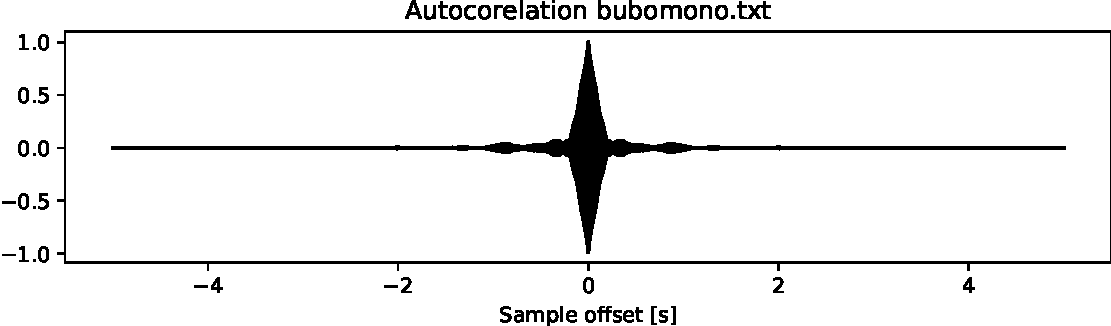
\includegraphics[width=12cm]{pdfs/bubomono.txt_acor.pdf}
    \vspace{10pt}
    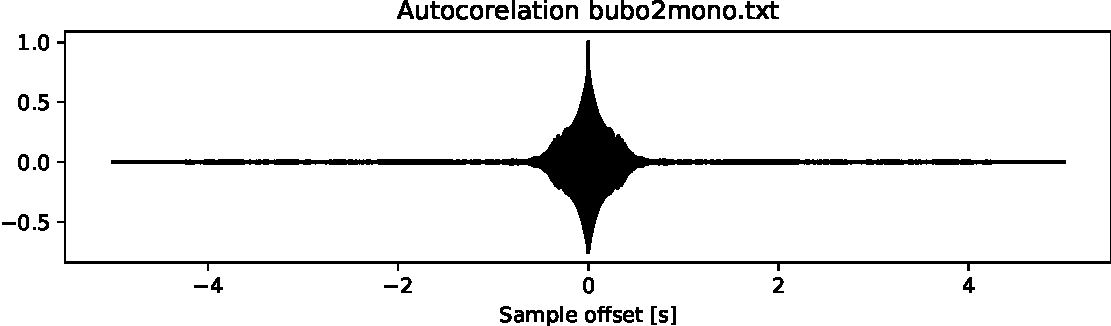
\includegraphics[width=12cm]{pdfs/bubo2mono.txt_acor.pdf}
    \caption{Avtokorelacija signala sov}
\end{figure}

Preden sem koreliral signal sem vektorja samplov normiral, tako da je
"najmočnejši" signal 1. To pomeni \[\|x\|_\infty = \max_i |x_i|\]

Poglejmo si še korelacije med sovami in posnetki:
\newpage
\begin{figure}[h]
    \centering
    \foreach \mix in {mix, mix1, mix2, mix22} {
        \foreach \sova in {bubomono, bubo2mono}{
            \includegraphics[width=8cm]{pdfs/cor_\mix.txt_\sova.txt.pdf}
        }
    }
    \caption{Korelacija sov in posnetkov iz narave}
\end{figure}
Tukaj je bila normalizacija drugače izbrana. Tukaj je bila narejena normalizacija korelacije. Če je varianca signala a $\sigma_a$,
potem je $ \mathbf{x} = \mathbf{x} / \left(\sigma_a \sigma_b |\mathbf{b}|\right)$. Sigma je izračunana z \verb|numpy.std()|.


Hitrosti so precej dolgčasno pričakovane ampak vseeno.
\begin{figure}[h]
    \centering
    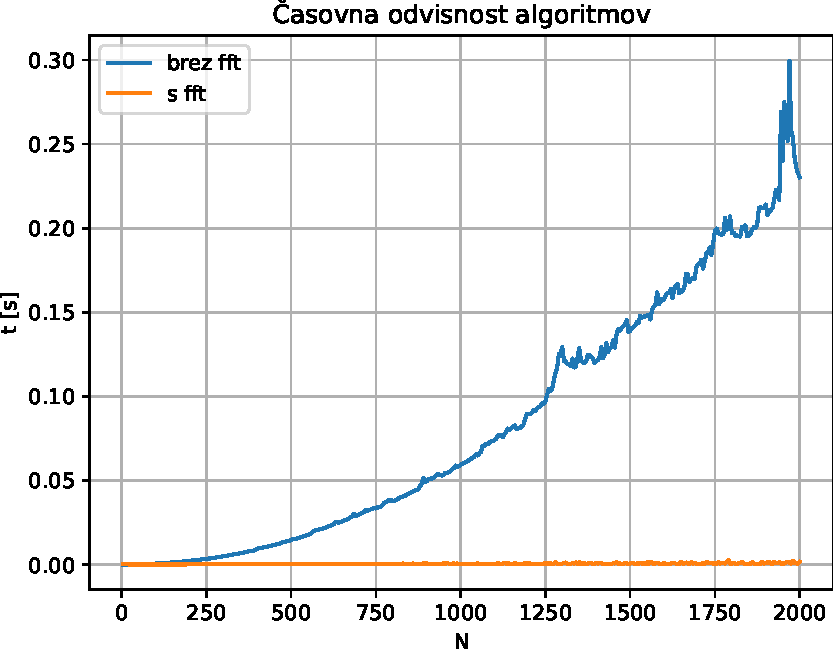
\includegraphics[width=8cm]{pdfs/cas-lin.pdf}
    \vspace{10pt}
    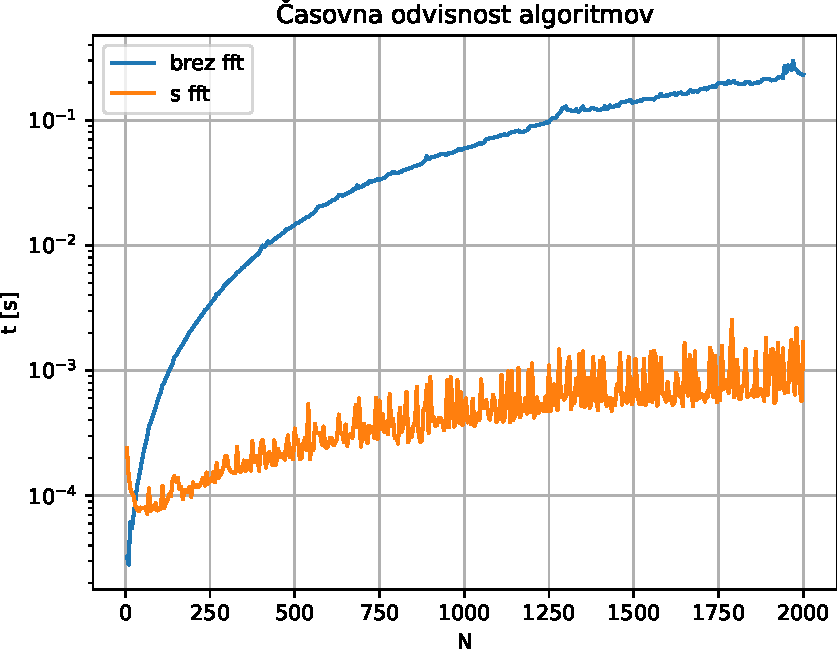
\includegraphics[width=8cm]{pdfs/cas-log.pdf}
    \caption{Hitrost algoritmov}
\end{figure}
\newpage
\section{Dodatna naloga}
Posnel sem dva človeka m in ž ko izgovarjata aaaaaaaaaaaa. Posnel sem jih tudi
ko bereta slovar. Gledal sem ali lahko spet zaznam ali gre za ž glas ali m glas.
Poglejmo si spektra njunega glasu.
\begin{figure}[h]
    \begin{center}
        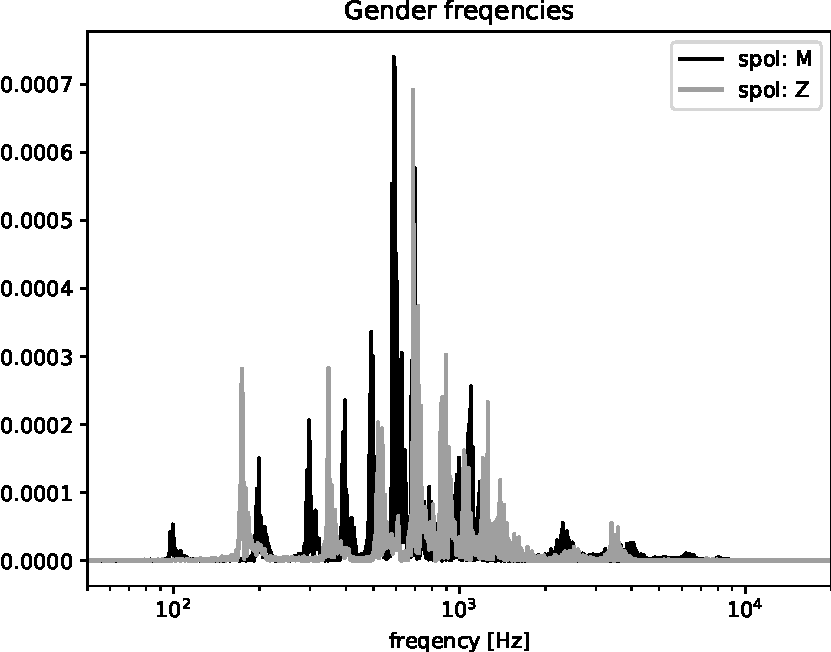
\includegraphics[width=12cm]{pdfs/fft_spol.pdf}
    \end{center}
    \caption{Barva glasu moškega in ženske}
\end{figure}

% Glasova sta bila prej normirana, saj je bil moški glas posnet bližje mikrofona.
% Poglejmo si zopet korelacijo med posnetki:
% \foreach \gender in {Z, M} {
%     \foreach \mix in {Glas\ 001, Glas\ 002}{
%         pdfs/cor_\gender_\mix.pdf 
%     }
% }
\begin{figure}[h]
    \begin{center}
        
    \foreach \gender in {Z, M} {%
        \foreach \mix in {001, 002} {%
            \includegraphics[width=8cm]{pdfs/cor_\gender_Glas\space\mix.pdf}%    
        }%
        \par
}%
    \end{center}
    
    \caption{Korelacija glasa človeka in posnetkov iz branja slovarja}
\end{figure}


\end{document}
